\documentclass{jsarticle}
\usepackage{amsmath, smssymb, amsfonts}
\usepackage{newtxtext, newtxmath}
\usepackage{latexsym}
\usepackage{mathrsfs}
\usepackage{mathtools}
\usepackage[dvipdfmx]{graphicx, xcolor}
\usepackage{float}
\usepackage{wrapfig}	% must be after float package.
\usepackage{subcaption}
\usepackage{booktabs}
\usepackage{url}
\usepackage{listings, jvlisting, color}

\definecolor{OliveGreen}{rgb}{0.0,0.6,0.0}
\definecolor{Orenge}{rgb}{0.89,0.55,0}
\definecolor{SkyBlue}{rgb}{0.28, 0.28, 0.95}
\lstset{
  language={C++}, % 言語の指定
  basicstyle={\ttfamily},
  identifierstyle={\small},
  commentstyle={\smallitshape},
  keywordstyle={\small\bfseries},
  ndkeywordstyle={\small},
  stringstyle={\small\ttfamily},
  frame={tb},
  breaklines=true,
  columns=[l]{fullflexible},
  numbers=left,
  xrightmargin=0zw,
  xleftmargin=3zw,
  numberstyle={\scriptsize},
  stepnumber=1,
  numbersep=1zw,
  lineskip=-0.5ex,
  keywordstyle={\color{SkyBlue}},     %キーワード(int, ifなど)の書体指定
  commentstyle={\color{OliveGreen}},  %注釈の書体
  stringstyle=\color{Orenge}          %文字列
}


\begin{document}

\title{ゼミ レポート 02}
\author{山田朔也}
\maketitle

\section{本レポートについて}
4月19日に行われたゼミにて出題された課題に対するレポートとなっている。
課題の内容は、熱伝導方程式を4次のルンゲクッタ法を用いて数値的に解き、4次のルンゲクッタ法による計算結果の性質を調べることになる。
また、初期条件などの条件設定は前回の課題に準拠する。

\section{4次のルンゲクッタ法について}
前回使用したオイラー法では1次の誤差が出ていたが、この誤差を減らすために4次のルンゲクッタ法を用いる。
前回のオイラー法では以下の微分方程式\ref{01}を式\ref{02}と近似計算していたが、
\begin{equation}
	\frac{dT}{dt} = f(t, T(i,t))	\label{01}
\end{equation}
\begin{equation}
	T(i,t+dt) = T(i,t) + dtf(t, T(i,t)) = T(i,t) + \frac{dt}{dx^2} (T(i-1,t) - 2T(i,t) + T(i+1,t))	\label{02}
\end{equation}
4次のルンゲクッタ法では、以下のように近似して計算をする。
\begin{align}
	T(i,t+dt) &= T(i,t) + \frac{dt}{6}(k_1 + 2k_2 + 2k_3 + k_4) \label{03} \\
	k_1		  &= f(t, T(i,t)) \notag \\
	k_2		  &= f(t+\frac{dt}{2}, (T(i,t) + \frac{dt}{2}k_1)) \notag \\
	k_3		  &= f(t+\frac{dt}{2}, (T(i,t) + \frac{dt}{2}k_2)) \notag \\
	k_4		  &= f(t+dt, (T(i,t) + dtk_3))	\notag
\end{align}
オイラー法では$t$と$t+dt$の間を単なる長方形とみなして計算していたが、
この4次のルンゲクッタ法では、$t$と$t+dt$の間に$t+dt/2$の点を置き、$f(t, T)$を二次関数に近似して計算していることになる。
そのため、単純なオイラー法よりも誤差が少なく計算する事ができる。

さらに、式\ref{03}を単純化すると以下のように表せる。
\begin{align}
	T(i,t+dt) &= T(i,t) + \frac{1}{6}(k_1 + 2k_2 + 2k_3 + k_4) \label{04} \\
	k_1		  &= dtf(t, T(i,t)) \notag \\
	k_2		  &= dttf(t+\frac{dt}{2}, (T(i,t) + \frac{1}{2}k_1)) \notag \\
	k_3		  &= dtf(t+\frac{dt}{2}, (T(i,t) + \frac{1}{2}k_2)) \notag \\
	k_4		  &= dtf(t+dt, (T(i,t) + k_3))	\notag
\end{align}
ここで、前回のレポートの際に作成した$f(t, T(i,t))$を計算する関数TTと、
$T(i,t)$と$f(t, T(i,t))$を足し合わせる関数vaddの2つを利用すると計算が可能となる。
アルゴリズムは以下のようになる。
\begin{enumerate}
	\item 各種初期条件を設定する。
	\begin{itemize}
		\item 棒の分割数$n$、またこれによって代表点間の距離$dx=\frac{1}{n}$が決定する。
		\item 温度の初期条件を$T$に設定する。
		\item 時間の刻み幅$dt$の決定
	\end{itemize}
	\item 初期条件と式\ref{04}から各代表点の$dt$後の状態を計算する。
	\begin{enumerate}
		\item 関数TTで$k_1$を計算する。
		\item 関数vaddを実行して得た値を関数TTに渡して$k_2$を計算する。
		\item 関数vaddを実行して得た値を関数TTに渡して$k_3$を計算する。
		\item 関数vaddを実行して得た値を関数TTに渡して$k_4$を計算する。
		\item $k_1, k_2, k_3, k_4$から$T(i, t+dt)$を計算する。
	\end{enumerate}
	\item 上の項目2を任意の回数行う。
\end{enumerate}

\section{問題1}
問題の内容は、熱伝導方程式を4次のルンゲクッタ法で解くプログラムを作成し、表の形式で出力して結果を確認するものだ。
まずは、以下に前述のアルゴリズムに則って作成したプログラムを記載する。

\begin{lstlisting}[H, caption=4次のルンゲクッタ法で解を得るプログラム, label=list01, language=C++]
	#include <stdio.h>
	#include <stdlib.h>
	#include <stdbool.h>
	
	int printout(int n, double* T, int t) {
		static bool IsFirst =true;
		int i = 0;
		if(IsFirst) {
			printf("time ");
			for(i = 0; i <= n; i++) {
				printf("T%d ", i);
			}
			printf("\n");
			IsFirst = false;
		}
	
		printf("%d*dt ", t);
		for (i = 0; i <= n; i++) {
			printf("%.4lf ", T[i]);
		}
		printf("\n");
	}
	
	int TT(double* T, double* k, double dx, double dt, int n) {
		int i = 0;
		k[0] = 0; k[n] = 0;
		for (i = 1; i < n; i++) {
			k[i] = dt*(T[i-1] - 2*T[i] + T[i+1])/(dx*dx);
		}
	}
	
	int vadd(double* T, double* T0, double* k, int n, double r) {
		int i = 0;
		for(i = 1; i < n; i++) {
			T[i] = T0[i] + k[i]*r;
		}
	}
	
	int vadd4(double* T, double* T0, double* k1, double* k2, double* k3, double* k4, int n) {
		int i = 0;
		for (i = 1; i < n; i++) {
			T[i] = T0[i] + (k1[i] + 2*k2[i] + 2*k3[i] + k4[i])/6;
		}
	}
	
	int main() {
		int n = 0;
		scanf("%d", &n);
	
		double dt = 0.0;
		scanf("%lf", &dt);
	
		double dx = 0.0;
		dx = (double)1.0 / (double)n;
		
		double T[n+1];
		double DT[n+1];
		double T0[n+1];
		double k1[n+1];
		double k2[n+1];
		double k3[n+1];
		double k4[n+1];
		
		int i = 0;
		for(i = 0; i <= n/2; i++) {
			T[i] = 2*dx*i;
			T[n-i] = T[i];
		}
		printout(n, T, 0);
	
		int t = 0;
		for (t = 1; t <= 10; t++) {
			int l = 0;
			for (l = 0; l <= n; l++) {
				T0[l] = T[l];
			}
			TT(T, k1, dx, dt, n);
			vadd(T, T0, k1, n, 0.5);
			TT(T, k2, dx, dt, n);
			vadd(T, T0, k2, n, 0.5);
			TT(T, k3, dx, dt, n);
			vadd(T, T0, k3, n, 1.0);
			TT(T, k4, dx, dt, n);
			vadd4(T, T0, k1, k2, k3, k4, n);
			printout(n, T, t);
		}
		return 0;
	}	
\end{lstlisting}

このプログラムの使用方法は、まずプログラムを実行した後、まずは分割数nを標準入力で入力。続いてdtも入力する。
するとそれを元に、初期条件及び、熱伝導方程式の数値的解を4次のルンゲクッタ法を用いて得ることができる。

結果の出力方法は、標準出力へとなっている。出力形式は以下の表\ref{結果01}のようになっている。
計算を行うにあたって、配列$T, T0, k1, k2, k3, k4$を用意する。
配列$T$は計算途中の最新の値を保持し、主に途中計算の保存用として使用する。
配列$T0$は計算途中で変化する前の、配列$T$の値を保存する目的で使用する。
配列$k1~k4$は式\ref{04}にある$k_1 ~ k_4$の値を保存する目的で使用する。
各関数の説明は以下のようになる。
\begin{itemize}
	\item 関数printout。配列$T$とその他の変数から、必要な情報を出力する。
	\item 関数TT。配列$T$に、各変数から受け取った値から計算した値を代入する。行う計算は$f(t, T(i,t))$の計算となっている。
	\item 関数vadd。配列$T$に、$T(i,t)$と$f(t, T(i,t))$を足し合わせた値を代入する関数。$f(t, T(i,t))$に係数$r$をかけられるようになっている。
	\item 関数vadd4。アルゴリズムの説明2-(e)の計算を実行している。計算結果は引数の配列$T$直接代入している。
\end{itemize}

このプログラムに$n=10, dt=0.001$を代入した時の結果は以下の表\ref{tab01}ようになった。
\begin{table}[H]
	\caption[出力結果]{作成したプログラムを$n=10$, $dt=0.001$で実行した出力結果}
	\label{tab01}
	\begin{center}
		\setlength{\tabcolsep}{3pt}
		\footnotesize
		\begin{tabular}{rccccccccccc}
			time & T0 & T1 & T2 & T3 & T4 & T5 & T6 & T7 & T8 & T9 & T10 \\
			0*dt & 0.0000 & 0.2000 & 0.4000 & 0.6000 & 0.8000 & 1.0000 & 0.8000 & 0.6000 & 0.4000 & 0.2000 & 0.0000 \\
			1*dt & 0.0000 & 0.2000 & 0.4000 & 0.5999 & 0.7982 & 0.9636 & 0.7982 & 0.5999 & 0.4000 & 0.2000 & 0.0000 \\
			2*dt & 0.0000 & 0.2000 & 0.4000 & 0.5996 & 0.7938 & 0.9333 & 0.7938 & 0.5996 & 0.4000 & 0.2000 & 0.0000 \\
			3*dt & 0.0000 & 0.2000 & 0.3999 & 0.5988 & 0.7876 & 0.9074 & 0.7876 & 0.5988 & 0.3999 & 0.2000 & 0.0000 \\
			4*dt & 0.0000 & 0.2000 & 0.3998 & 0.5976 & 0.7802 & 0.8850 & 0.7802 & 0.5976 & 0.3998 & 0.2000 & 0.0000 \\
			5*dt & 0.0000 & 0.2000 & 0.3995 & 0.5958 & 0.7721 & 0.8653 & 0.7721 & 0.5958 & 0.3995 & 0.2000 & 0.0000 \\
			6*dt & 0.0000 & 0.1999 & 0.3991 & 0.5936 & 0.7636 & 0.8476 & 0.7636 & 0.5936 & 0.3991 & 0.1999 & 0.0000 \\
			7*dt & 0.0000 & 0.1998 & 0.3986 & 0.5909 & 0.7549 & 0.8316 & 0.7549 & 0.5909 & 0.3986 & 0.1998 & 0.0000 \\
			8*dt & 0.0000 & 0.1997 & 0.3978 & 0.5879 & 0.7462 & 0.8169 & 0.7462 & 0.5879 & 0.3978 & 0.1997 & 0.0000 \\
			9*dt & 0.0000 & 0.1995 & 0.3969 & 0.5846 & 0.7374 & 0.8032 & 0.7374 & 0.5846 & 0.3969 & 0.1995 & 0.0000 \\
			10*dt & 0.0000 & 0.1993 & 0.3959 & 0.5810 & 0.7288 & 0.7905 & 0.7288 & 0.5810 & 0.3959 & 0.1993 & 0.0000 \\
		\end{tabular}
	\end{center}
\end{table}
この結果は、オイラー法を使用した際の結果とほぼ一致している。以下の表\ref{tab02}オイラー法を使用した際の結果の表と成る。
\begin{table}[H]
	\caption[出力結果]{作成したプログラムを$n=10$, $dt=0.001$で実行した出力結果}
	\label{tab02}
	\begin{center}
		\setlength{\tabcolsep}{3pt}
		\footnotesize
		\begin{tabular}{rccccccccccc}
			time & T0 & T1 & T2 & T3 & T4 & T5 & T6 & T7 & T8 & T9 & T10	\\
			0*dt & 0.0000 & 0.2000 & 0.4000 & 0.6000 & 0.8000 & 1.0000 & 0.8000 & 0.6000 & 0.4000 & 0.2000 & 0.0000	\\
			1*dt & 0.0000 & 0.2000 & 0.4000 & 0.6000 & 0.8000 & 0.9600 & 0.8000 & 0.6000 & 0.4000 & 0.2000 & 0.0000	\\
			2*dt & 0.0000 & 0.2000 & 0.4000 & 0.6000 & 0.7960 & 0.9280 & 0.7960 & 0.6000 & 0.4000 & 0.2000 & 0.0000	\\
			3*dt & 0.0000 & 0.2000 & 0.4000 & 0.5996 & 0.7896 & 0.9016 & 0.7896 & 0.5996 & 0.4000 & 0.2000 & 0.0000	\\
			4*dt & 0.0000 & 0.2000 & 0.4000 & 0.5986 & 0.7818 & 0.8792 & 0.7818 & 0.5986 & 0.4000 & 0.2000 & 0.0000	\\
			5*dt & 0.0000 & 0.2000 & 0.3998 & 0.5971 & 0.7732 & 0.8597 & 0.7732 & 0.5971 & 0.3998 & 0.2000 & 0.0000	\\
			6*dt & 0.0000 & 0.2000 & 0.3996 & 0.5950 & 0.7643 & 0.8424 & 0.7643 & 0.5950 & 0.3996 & 0.2000 & 0.0000	\\
			7*dt & 0.0000 & 0.1999 & 0.3992 & 0.5924 & 0.7551 & 0.8268 & 0.7551 & 0.5924 & 0.3992 & 0.1999 & 0.0000	\\
			8*dt & 0.0000 & 0.1999 & 0.3986 & 0.5893 & 0.7460 & 0.8125 & 0.7460 & 0.5893 & 0.3986 & 0.1999 & 0.0000	\\
			9*dt & 0.0000 & 0.1998 & 0.3978 & 0.5859 & 0.7370 & 0.7992 & 0.7370 & 0.5859 & 0.3978 & 0.1998 & 0.0000	\\
			10*dt & 0.0000 & 0.1996 & 0.3968 & 0.5822 & 0.7281 & 0.7867 & 0.7281 & 0.5822 & 0.3968 & 0.1996 & 0.0000	\\
		\end{tabular}
	\end{center}
\end{table}%
このことから、この計算を行うプログラムはおおよそあっていると考えられる。

\section{問題2}
問題の内容は、問題1で計算した結果(表\ref{tab01})をgnuplotを用いてグラフ化することとなっている。
以下にグラフ化したものを図\ref{fig01}として以下に記載する。
\begin{figure}[H]
	\centering
	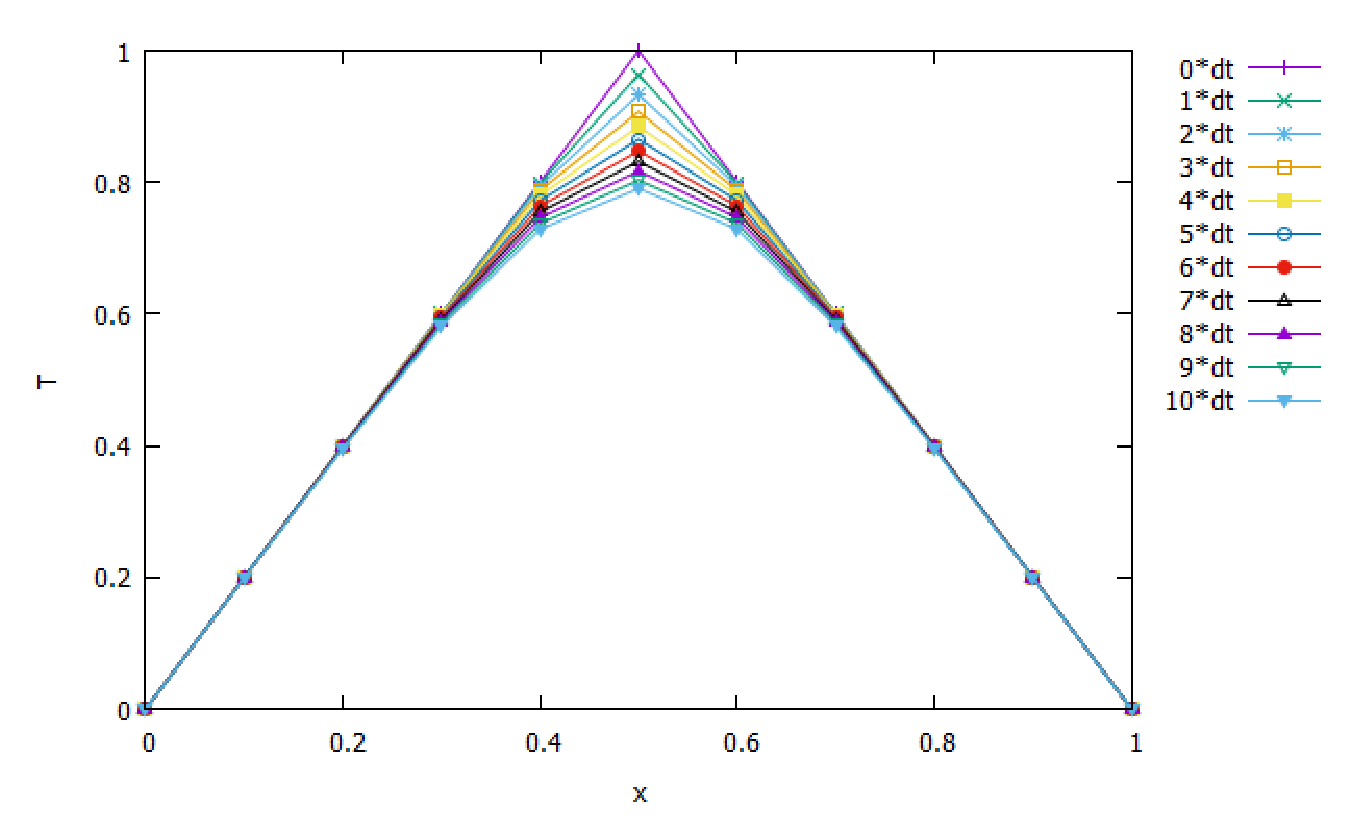
\includegraphics[width=14cm]{pic01.eps}
	\caption{表\ref{tab01}をグラフ化した図}
	\label{fig01}
\end{figure}

\section{問題3}
問題の内容は$dt$を変化させてを変化させて計算を行い、中央の点における温度変化に対する$dt$の影響を調べる。また結果をオイラー法と比較する。

まず、$n=10$に$n$の値を固定した後、$dt$を0.001から0.001ずつ変化させて、計算を行っていった。
このとき、$dt=0.008$のときにはじめて計算が破綻した。
その時の実行結果のグラフが以下の図\ref{fig02}となる。
図のように明らかに計算が破綻している事がわかる。
\begin{figure}[H]
	\centering
	\begin{subfigure}{0.9\columnwidth}
		\centering
		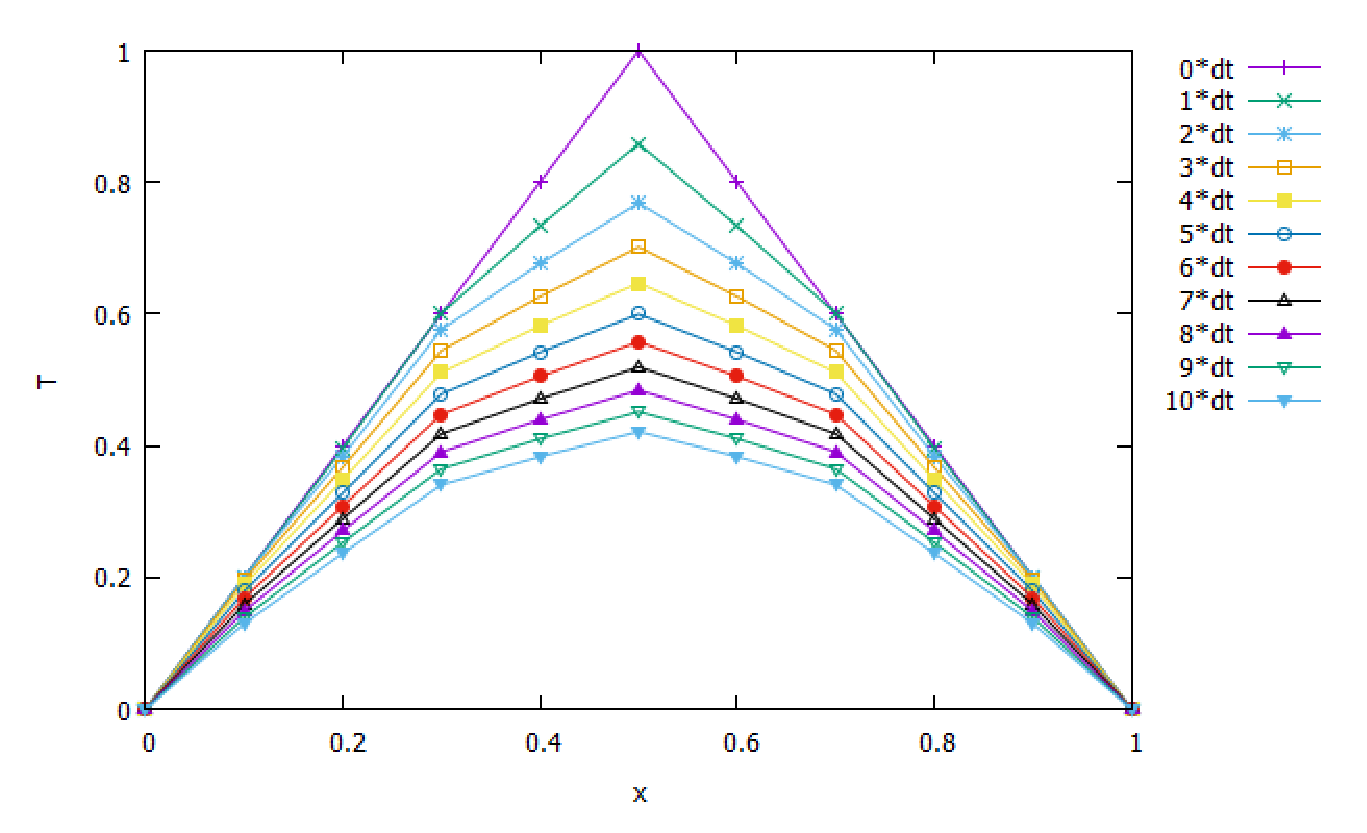
\includegraphics[width=\columnwidth]{pic02.eps}
		\caption{$dt=0.007$の時の実行結果}
	\end{subfigure}
	\begin{subfigure}{0.9\columnwidth}
		\centering
		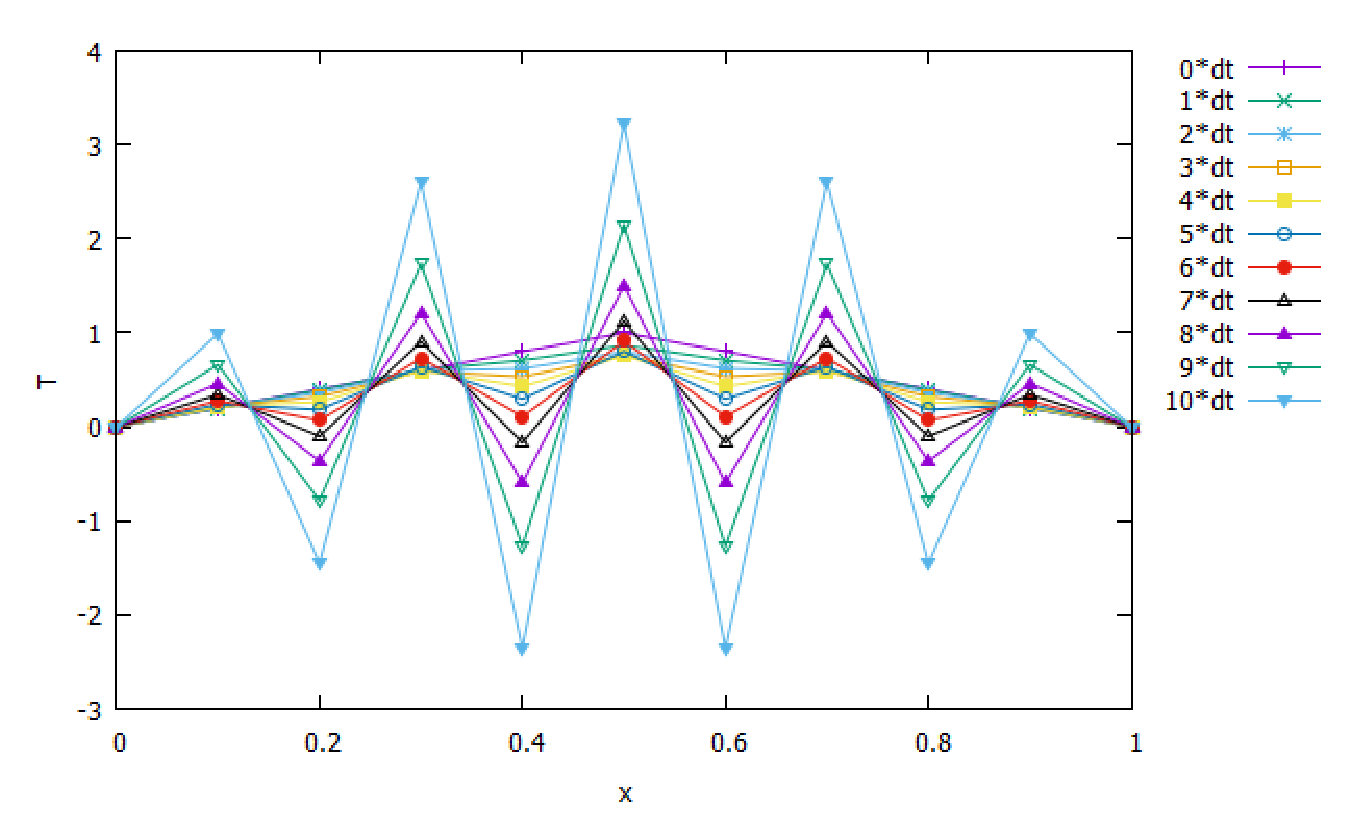
\includegraphics[width=\columnwidth]{pic03.eps}
		\caption{$dt=0.008$の時の実行結果}
	\end{subfigure}
	\label{fig02}
	\caption{0.001ずつ増加させたときの実行結果}
\end{figure}
次に、$dt$を0.0070から0.0001ずつ増やして計算を行っていく。
この時、ループ回数を10ではあまり変化が見られなかったため、ループ回数を100回にして計算を行った。
計算した結果0.0071で、計算結果が本来至らないはずの負の値の温度を示していた。
以下の図\ref{fig03}に$dt=0.0070$のときと$dt=0.0071$の時の比較を載せている。
\begin{figure}[H]
	\centering
	\begin{subfigure}{0.9\columnwidth}
		\centering
		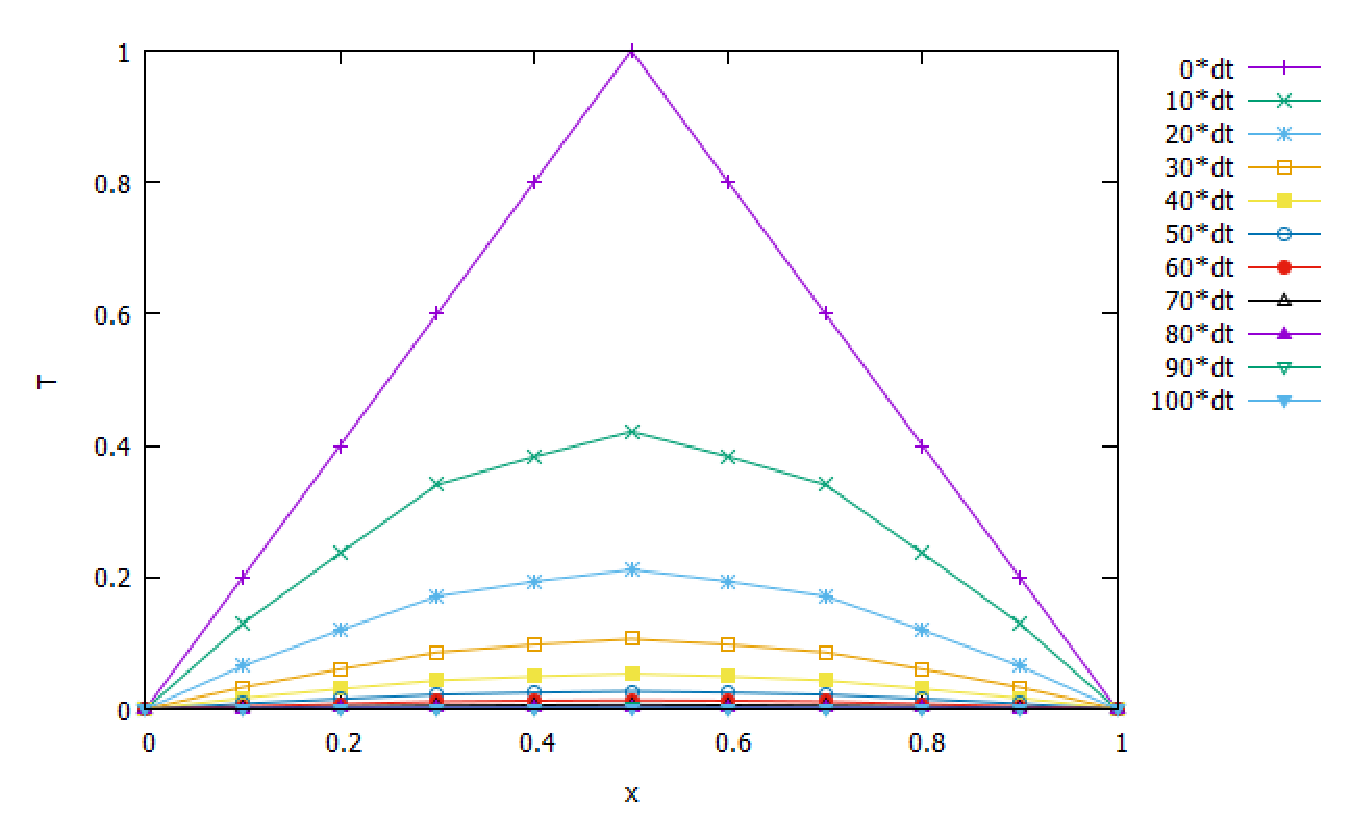
\includegraphics[width=\columnwidth]{pic04.eps}
		\caption{$dt=0.0070$の時の実行結果}
	\end{subfigure}
	\begin{subfigure}{0.9\columnwidth}
		\centering
		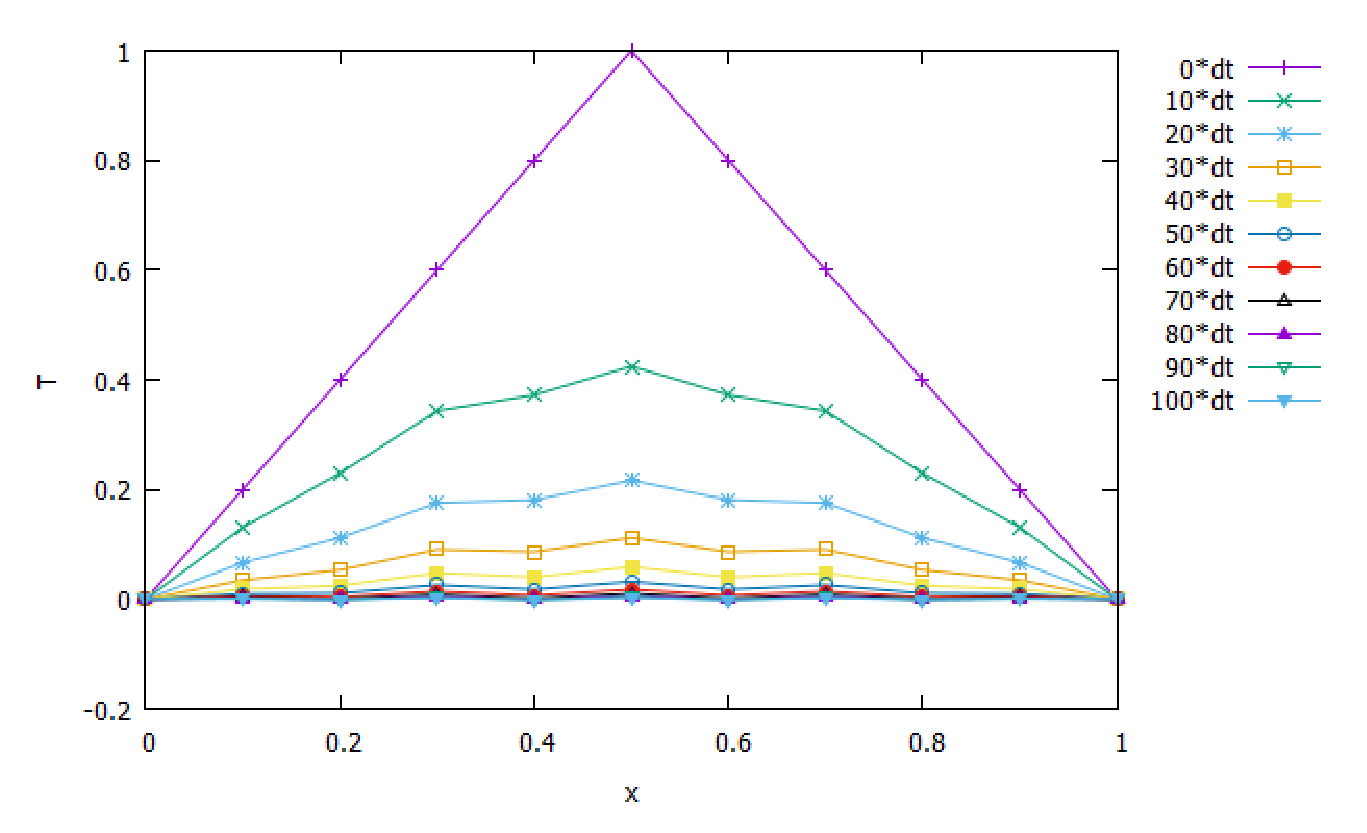
\includegraphics[width=\columnwidth]{pic05.eps}
		\caption{$dt=0.0071$の時の実行結果}
	\end{subfigure}
	\label{fig03}
	\caption{$dt$を0.0001ずつ増加させたときの実行結果}
\end{figure}
このことから、$n=10$のときは$dt=0.007$が正しく計算可能な限界点だと見て取れる。
また、オイラー法では0.0052から計算が破綻していたことを考えると、たしかにルンゲクッタ法を導入したほうが、
初期設定の値の設定可能範囲が広がることがわかる。

\section{問題4}
問題の内容は$n$を変化させてを変化させて計算を行い、中央の点における温度変化に対する$n$の影響を調べる。また結果をオイラー法と比較する。

まず、$dt=0.001$に$dt$の値を固定した後、$n$を10から1ずつ増やして、計算を行っていった。
このとき、$n=27$のときにはじめて計算が破綻した。
また、計算におけるループ回数は10ではあまり変化が見られなかったため、ループ回数を100回にして計算を行った。
以下の図\ref{fig04}に$n=26$のときと$n=27$の時の比較を載せている。
\begin{figure}[H]
	\centering
	\begin{subfigure}{0.9\columnwidth}
		\centering
		
\includegraphics[width=\columnwidth]{pic06.eps}
		\caption{$n=26$の時の実行結果}
	\end{subfigure}
	\begin{subfigure}{0.9\columnwidth}
		\centering
		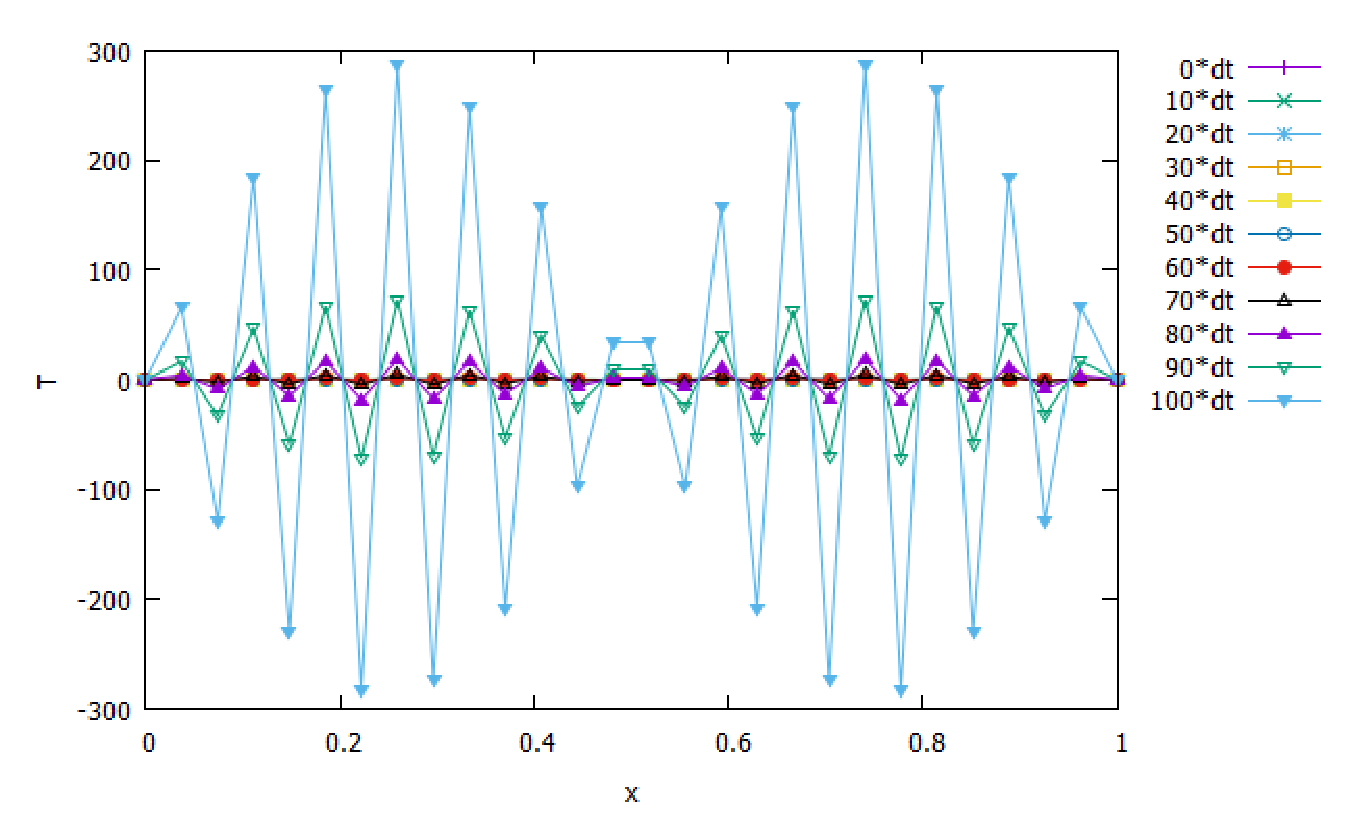
\includegraphics[width=\columnwidth]{pic07.eps}
		\caption{$n=27$の時の実行結果}
	\end{subfigure}
	\label{fig04}
	\caption{$n$を1ずつ増加させたときの実行結果}
\end{figure}
このことから、$dt=0.001$のときは$n=26$が正しく計算可能な限界点だと見て取れる。
また、オイラー法では$n=24$から計算が破綻していたことを考えると、たしかにルンゲクッタ法を導入したほうが、
初期設定の値の設定可能範囲が広がることがわかる。

\section{問題5}
問題の内容は、$dt,n$を共に変化させて計算を行い、計算が破綻しない条件を探すことである。

まず、$n$の値を$8~32$の範囲で変化させ、その中で更に$dt$を$dt=0.0001$から$0.0001$ずつ増やしつつ、
計算が破綻する直前の値を調べた。
また、計算の破綻は、どこかの代表点が負の温度に達した場合とする。
それらの値を、$n$の値を横軸に、$dt$の値を縦軸に取ると以下の図\ref{fig05}ようなグラフになった。
\begin{figure}[H]
	\centering
	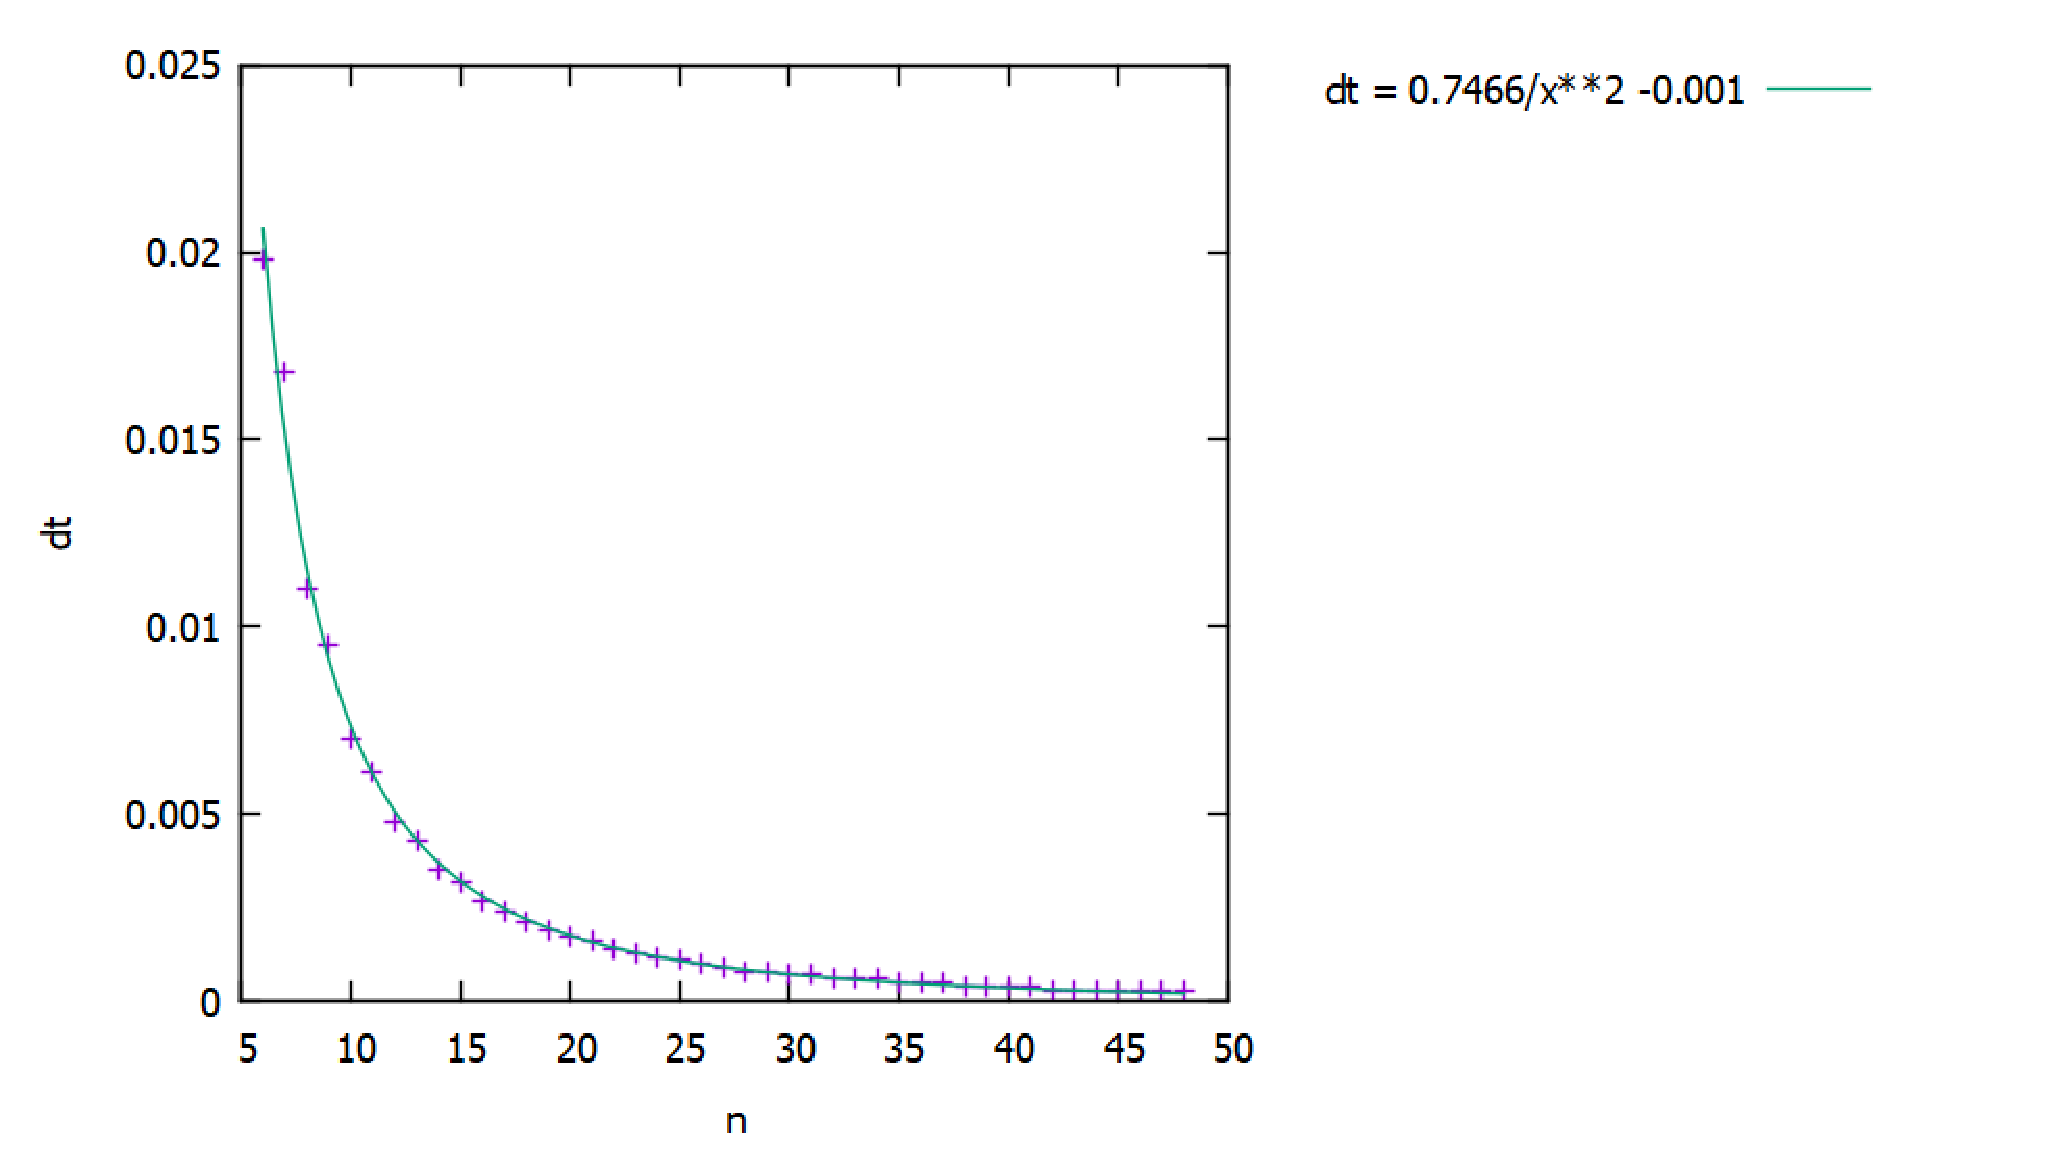
\includegraphics[width=14cm]{pic08.eps}
	\caption{各$n$の値に対して、ちょうど計算が破綻しない$dt$の値とその近似曲線}
	\label{fig05}
\end{figure}
この図にもあるように、ちょうど計算が破綻しない$dt$の値から近似曲線を取ると以下のような式になった。
\begin{equation}
	dt = \frac{0.7466}{x^2} - 0.001	\label{05}
\end{equation}
このことから、解が安定して求められる条件は、$dt$の値が式\ref{05}の右辺の値を超えなければ良いと解る。

\section{問題6}
問題の内容は、ルンゲクッタ法で熱伝導方程式を数値的に解くことを、二次元に拡張することである。

2次元に拡張した際に異なってくることは、式\ref{01}における$f(t, T(i,t))$の中身となる。
1次元においては、前回のレポートに記載した通り、
\begin{equation}
	f(t, T(i,t)) = \frac{T(i-1,t) - 2T(i,t) + T(i+1,t)}{dx^2}	\label{06}
\end{equation}
となるが、2次元に拡張すると、上記の式は以下のようになる。
\begin{equation}
	f(t, T(i,j,t)) = \frac{T(i-1,j,t) - 2T(i,j,t) + T(i+1,j,t)}{dx^2} + \frac{T(i,j-1,t) - 2T(i,j,t) + T(i,j+1,t)}{dy^2}
	\label{07}
\end{equation}
これを今まで使用してきたアルゴリズムに適応すればよい。
なお、今回の初期条件は、2次元空間上に縦横長さ1の板を想定する。
その上で、その板の周囲の境界の温度は常に0とする。
それ以外の点は以下のようになる。
\begin{equation}
	\label{08}
	T(x,y,0) = \begin{cases}
		4xy & (0 \leqq x \leqq \frac{1}{2}, 0 \leqq y \leqq \frac{1}{2}) \\
		4(1-x)y & (\frac{1}{2} \leqq x \leqq 1, 0 \leqq y \leqq \frac{1}{2}) \\
		4x(1-y) & (0 \leqq x \leqq \frac{1}{2}, \frac{1}{2} \leqq y \leqq 1) \\
		4(1-x)(1-y) & (\frac{1}{2} \leqq x \leqq 1, \frac{1}{2} \leqq y \leqq 1)
	\end{cases}
\end{equation}

また、計算する際には板を$n\times n$のグリッドに分割し、これにより$dx, dy$が決定する。
記載した以外のことは1次元に準拠する。

以下に前述のアルゴリズムに則って作成したプログラムを記載する。
\begin{lstlisting}[H, caption=2次元空間での4次のルンゲクッタ法で解を得るプログラム, label=list02, language=C++]
	#include <stdio.h>
	#include <stdlib.h>
	#include <stdbool.h>
	
	int printout(int n, double T[][11], double saveT[][11][11], int t, int issave) {
		int i = 0, j = 0, k = 0;
		double dx = (double)1.0 / (double)n;
		if (issave) {
			for (i = 0; i <= n; i++) {
				for (j = 0; j <= n; j++) {
					saveT[i][j][t] = T[i][j];
				}
			}
		} else {
			for (i = 0; i <= n; i++) {
				for (j = 0; j <= n; j++) {
					//printf("test");
					printf("%.4lf %.4lf ", dx*i, dx*j);
					for (k = 0; k <= 10; k++) {
						//printf("a");
						printf("%.4lf ", saveT[i][j][k]);
					}
					printf("\n");
				}
				printf("\n");
			}
		}
	}
	
	int TT(double T[][11], double k[][11], double dx, double dt, int n) {
		int i = 0, j = 0;
		for (i = 0; i <= n; i++) {
			k[0][i] = 0; k[n][i] = 0; k[i][0] = 0; k[i][n] = 0; 
		}
		for (i = 1; i < n; i++) {
			for (j = 1; j < n; j++) {
				k[i][j] = dt*(T[i-1][j] - 2*T[i][j] + T[i+1][j] + T[i][j-1] - 2*T[i][j] + T[i][j+1])/(dx*dx);
			}
		}
	}
	
	int vadd(double T[][11], double T0[][11], double k[][11], int n, double r) {
		int i = 0, j = 0;
		for(i = 1; i < n; i++) {
			for (j = 1; j < n; j++) {
				T[i][j] = T0[i][j] + k[i][j]*r;
			}
		}
	}
	
	int vadd4(double T[][11], double T0[][11], double k1[][11], double k2[][11], double k3[][11], double k4[][11], int n) {
		int i = 0, j = 0;
		for (i = 1; i < n; i++) {
			for (j = 1; j < n; j++) {
				T[i][j] = T0[i][j] + (k1[i][j] + 2*k2[i][j] + 2*k3[i][j] + k4[i][j])/6;
			}
		}
	}
	
	int main() {
		int n = 10;
	
		double dt = 0.001;
	
		double dx = 0.0;
		dx = 1.0 / (double)n;
	
		double T[n+1][n+1];
		double T0[n+1][n+1];
		double k1[n+1][n+1];
		double k2[n+1][n+1];
		double k3[n+1][n+1];
		double k4[n+1][n+1];
		double saveT[n+1][n+1][11];
	
		int i = 0, j = 0;
		for(i = 0; i <= n/2; i++) {
			for (j = 0; j <= n/2; j++) {
				T[i][j] = 4*dx*dx*i*j;
				T[n-i][n-j] = T[i][j];
				T[i][n-j] = T[i][j];
				T[n-i][j] = T[i][j];
			}
		}
		printout(n, T, saveT, 0, 1);
	
		int t = 0;
		for (t = 1; t <= 100; t++) {
			for (i = 0; i <= n; i++) {
				for (j = 0; j <= n; j++) {
					T0[i][j] = T[i][j];
				}
			}
			TT(T, k1, dx, dt, n);
			vadd(T, T0, k1, n, 0.5);
			TT(T, k2, dx, dt, n);
			vadd(T, T0, k2, n, 0.5);
			TT(T, k3, dx, dt, n);
			vadd(T, T0, k3, n, 1.0);
			TT(T, k4, dx, dt, n);
			vadd4(T, T0, k1, k2, k3, k4, n);
			if (t % 10 == 0) {
				printout(n, T, saveT, t/10, 1);
			}
		}
	
		printout(n, T, saveT, 0, 0);
		return 0;
	}
\end{lstlisting}

これを$n=10,dt=0.001$で実行した際の実行結果は以下の図\ref{fig06}のようになった。
\begin{figure}[H]
	\centering
	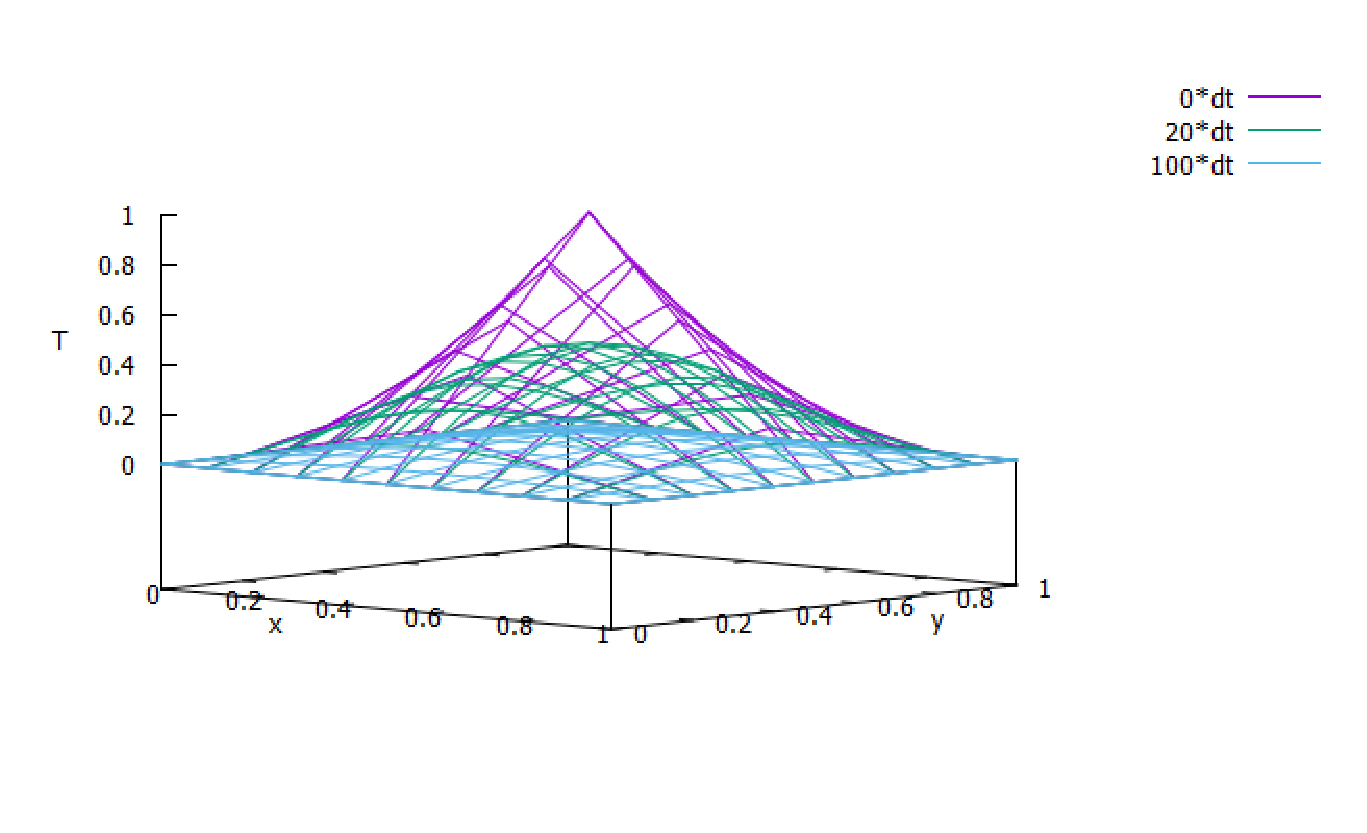
\includegraphics[width=14cm]{pic09.eps}
	\caption{4次のルンゲクッタ法を2次元に拡張した際の実行結果}
	\label{fig06}
\end{figure}



\section{参考文献}

\begin{itemize}
  \item 配布されたテキスト
  \item 前回のレポート
\end{itemize}

\end{document}